\documentclass{article}
\usepackage[utf8]{inputenc}
\usepackage{tikz}

\begin{document}
  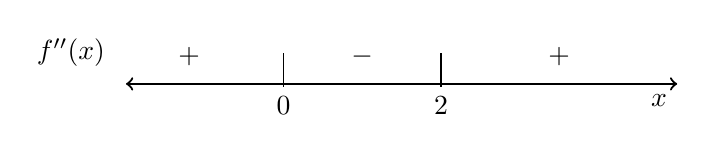
\begin{tikzpicture} 
    \draw[thick](-2.7,0.7)node[anchor=north]{$f''(x)$};
    \draw[thick,<->] (-2,0) -- (5,0) node[anchor=north east] {$x$};
    \foreach \x in {0,2}
       \draw (\x cm,1.1em) -- (\x cm,-1pt) node[anchor=north] {$\x$};
    \draw[thick] (-1.2,0.6)node[anchor=north]{$+$};
    \draw[thick] (1,0.6)node[anchor=north]{$-$};
    \draw[thick] (3.5,0.6)node[anchor=north]{$+$};
  \end{tikzpicture} 
\end{document}
